\chapter{Experiments}\label{cha:result}

This Chapter first describes the experiment to evaluate the algorithm and then presents the results.

\section{Evaluation measures}

To be able to compare the results from the different feature descriptors with each other, it is crucial to have some kind of evaluation measurement. The most common measurements for binary classifiers are based on the confusion matrix \cite{sokolova2009systematic}. 

The confusion matrix displays the result from a classifier consist of four values:

\begin{itemize}
	\item True positive (TB)\\
	The samples which were labeled as class one has also been predicted to belong to class one.
	
	\item True negative (TN)\\
	The samples which were labeled as class two has also been predicted to belong to class two.
	
	\item False positive (FP)\\
	Samples that were incorrectly assigned to class one.
	
	\item False negative (FN)\\
	Samples that were incorrectly assigned to class two.
\end{itemize}

\FloatBarrier
\begin{figure}[!h]
	\centering
	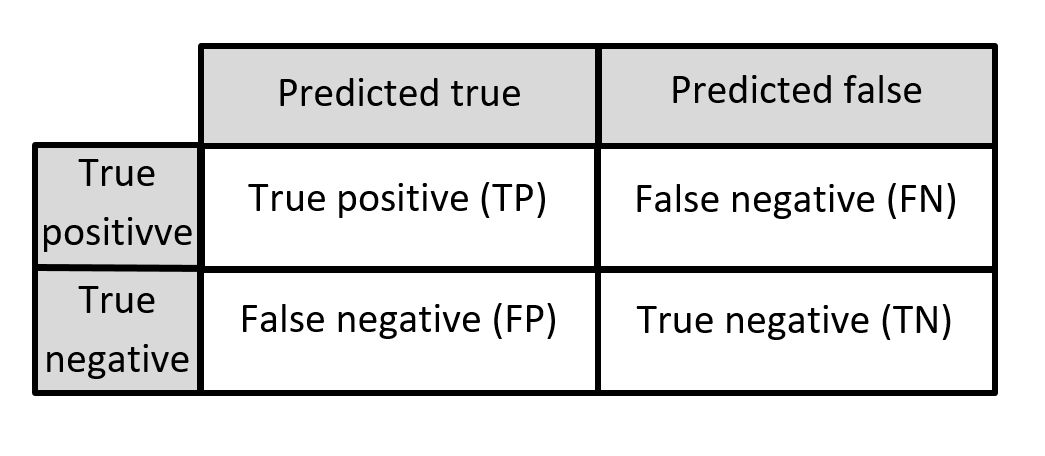
\includegraphics[width=\textwidth*3/4,height=\textheight*3/4,keepaspectratio]{confusion_matrix.PNG}
	\caption{Confusion matrix
		\label{fig:confusion}}
\end{figure} 
\FloatBarrier

From the confusion matrix, a collections of performance measurement can be calculated. This master thesis will use three values: accuracy \cref{eq:accuracy}, precision \cref{eq:precision} and recall \cref{eq:recall}. Accuracy show the overall effectiveness of the classifier. Precision show class agreement of the data labels with the positive labels given by the classifier. Recall show the effectiveness of a classifier to identify positive labels

\begin{equation} \label{eq:accuracy}
\text{Accuracy} \: [\%] = \frac{\text{TP} + \text{TN}}{\text{TP}+\text{TN}+\text{FP}+\text{FN}}
\end{equation}

\begin{equation} \label{eq:precision}
\text{Precision} \: [\%] = \frac{\text{TP}}{\text{TP}+\text{FP}}
\end{equation}
\begin{equation} \label{eq:recall}
\text{Recall} \: [\%] = \frac{\text{TP}}{\text{TP}+\text{FN}}
\end{equation}

%\subsection{Cross validation}
%
%In order to avoid overfitting and get a reliable performance value, one often use a method called cross validation. Cross validation is when the data is split up into $k$-subsets and one of them is used as test data while $k -1$ are used as training data. See \cref{fig:cross_validation} for a schematic overview of a five-fold cross validations procedure.  




\section{Experiment setup}

The experiment was set such that the image set was processed by the algorithm with 11 different thresholds values, $h_{FRS}$, for the FRS-image. The $h_{FRS}$ ranged from $0.05$ to $0.15$. The output was compared to the ground truth. A correct detection was defined as all detections which overlaps with an annotated mark. This definition has been chosen since some of the detections can be very small. Also, since candidates with a area larger than 1000 pixels has been eliminated, no overly large candidates can give correct detections.   

The $h_{FRS}$-value which gives the best recall value was used to evaluate the elimination process of the candidates. This was done by calculating the precision and recall values before the different elimination steps. The results is displayed in \cref{fig:results_bar_frs}.

To evaluate how the elimination process is working, the recall and precision values after each elimination step. These results can be observed in \cref{fig:results_bar_elimniation}.

To evaluate the facial mark classifier, a cross validation of the 506 annotated mark were performed. 100 marks was chosen at random to be used as test marks while the remaining marks was used for training the SVM, see \cref{fig:cross_validation}. This was repeated until all the marks had been used as test marks.

In order to find the best set of descriptive features from \cref{table:feature_sets}, the classifier was trained for each set of features. The parameters $C$ and $\gamma$ was optimized for each set.  

\FloatBarrier
\begin{figure}[!h]
	\centering
	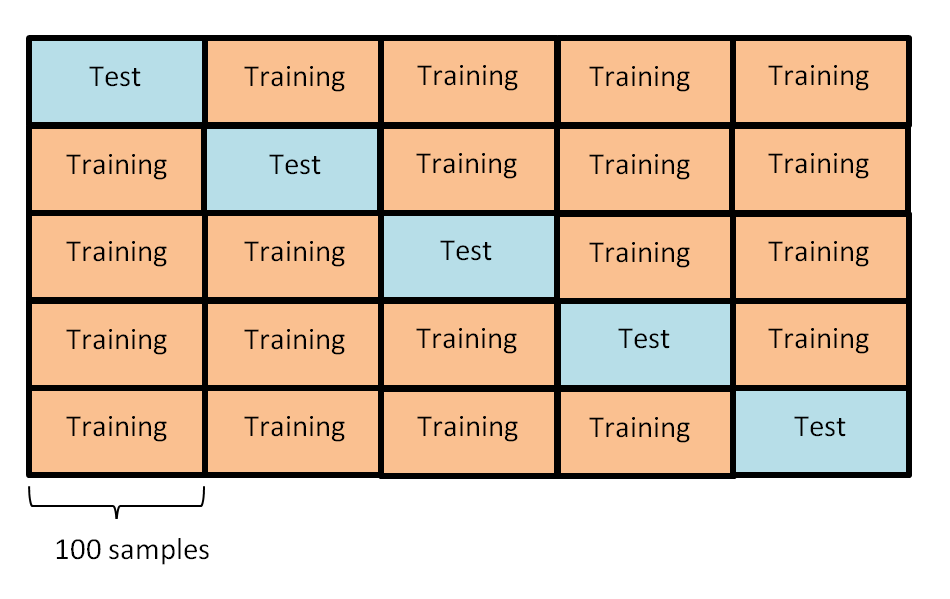
\includegraphics[width=\textwidth*3/4,height=\textheight*3/4,keepaspectratio]{cross_validation.PNG}
	\caption{Cross validation
		\label{fig:cross_validation}}
\end{figure} 
\FloatBarrier


%In order to find the best $C$-value and $\gamma$-value for the mark classifier, the parameters are varied over a rough interval to narrow down the search. Afterwards, a more fine interval is used to find the best parameters. This has been shown by Chih-Wei et. al. \cite{svm_guide}  to be an effective method compared to a more random selection of parameters which is often used by people unfamiliar to SVM. 

\section{Results}

This section will present the results from experiment described above. The result is divided into two parts: Detector and Classifier. 

\subsection{Detector}

Here the results from the facial mark detector is presented. In the \cref{fig:results_bar_frs}, the precision and recall for different $h_{FRS}$-value can be examined. The precision corresponds to the white bar and the recall corresponds to the black bar. Note that this is only the detections of facial mark and no classification between permanent and non-permanent marks. 

\FloatBarrier
\begin{figure}[h!]
	\centering
	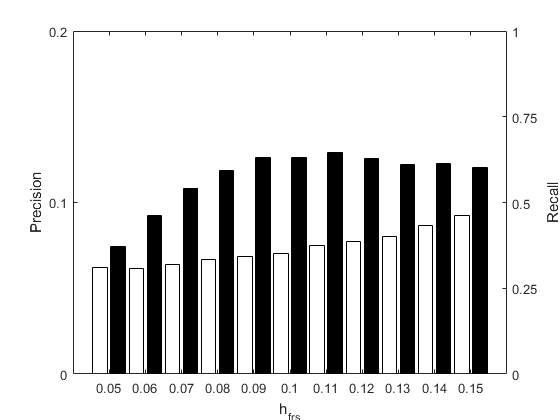
\includegraphics[width=\textwidth*3/4,height=\textheight*3/4,keepaspectratio]{results_bar_frs}
	\caption{Detection results from the algorithm with different $h_{frs}$-values. The white bars represents the precision value and the black bars represents recall value.  \label{fig:results_bar_frs}}
\end{figure}
\FloatBarrier

As one can see, the precision increases with higher $h_{FRS}$-value without affecting the recall substantially. This is means that the number of candidates decreases with a growing $h_{FRS}$-value. Thus, a small $h_{FRS}$-value results in a large number of candidates while a larger value gives fewer candidates.

Note that the number of candidates found by the detector decreases with a larger $h_{FRS}$-value, see \cref{fig:hair_vs_hair}. The size of the candidates also decreases which could explain the increase of recall in \cref{fig:results_bar_frs}. The algorithm finds different kind of candidates for small $h_{FRS}$-values. 

\FloatBarrier
\begin{figure}[h!]
	\centering
	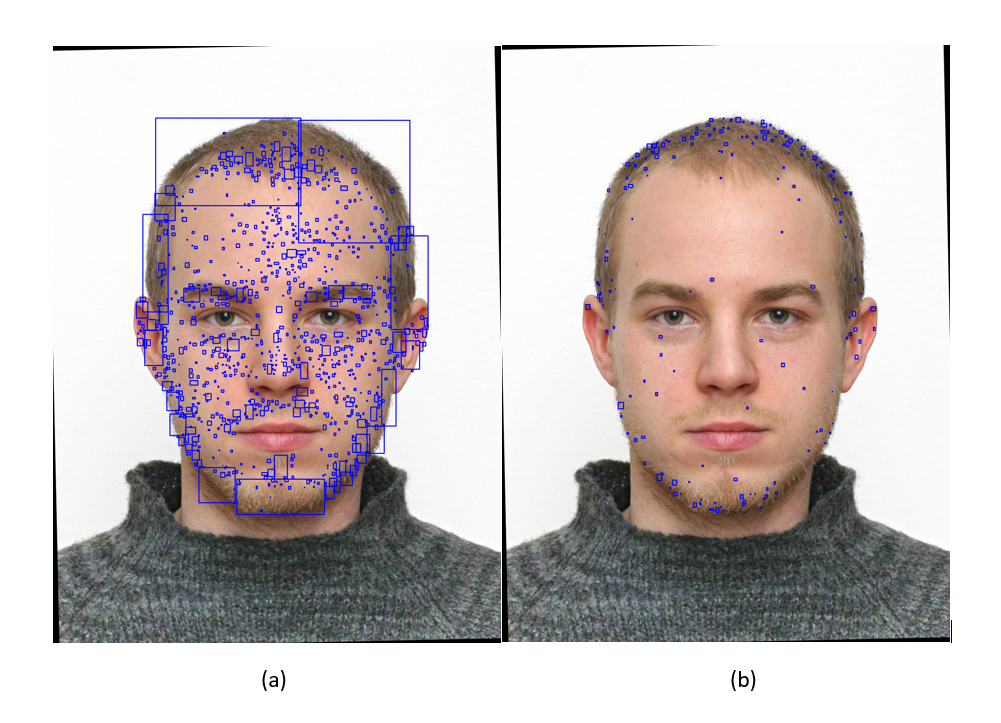
\includegraphics[width=\textwidth*3/4,height=\textheight*3/4,keepaspectratio]{hair_vs_hair}
	\caption{Candidate detection before post-processing, (a) with small $h_{hair}$-value, (b) with large $h_{hair}$-value,   \label{fig:hair_vs_hair}}
\end{figure}
\FloatBarrier

In \cref{fig:results_bar_elimniation}, it is possible to see the effects of the different elimination steps. As before, the white bar represent the precision and the black bar represents the recall. The first pair is the result just after the candidate detection and the second pair is the result after the blob detector. Furthermore, the third pair is after the hair eliminator and the last pair is after the size eliminator. 

\FloatBarrier
\begin{figure}[h!]
	\centering
	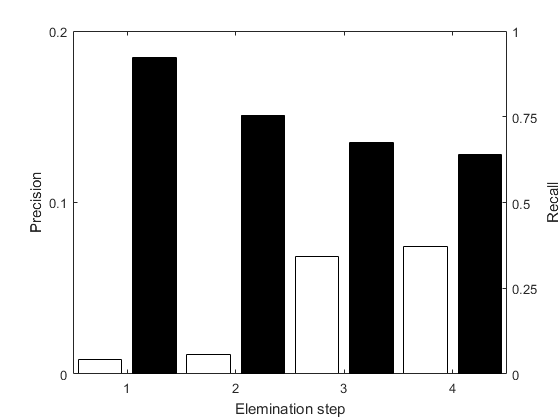
\includegraphics[width=\textwidth*3/4,height=\textheight*3/4,keepaspectratio]{results_bar_elimniation}
	\caption{Detection results from the algorithm  after different candidate elimination steps. 1 = before elimination, 2 = after blob-elimination, 3 = after hair-elimination, 4 = after size-elimination. The white bars represents the precision value and the black bars represents recall value.  \label{fig:results_bar_elimniation}}
\end{figure}
\FloatBarrier

It is obvious that the different eliminators are essential for the algorithm. The hair eliminator improves the precision the most while the blob detector worsens the recall the most.     


In \cref{fig:all_detections} below one can observe all the candidates found by the detector before post-processing. The candidates are shown as blue bounding boxes and the annotated facial marks for this image is show as red bounding boxes. There are many false detections in the hair and the beard which is some of the problems identified in this master thesis. 

After the post-processing, \cref{fig:all_hits}, almost all the false detection has been eliminated but some of them remain. The remaining false detection are located in the beard and hair. Some bounding boxes are around skin marks which has not been deemed of interest by the forensics at NFC. 

\FloatBarrier
\begin{figure}[h]
	\centering
	\includegraphics[width=\textwidth*4/10,height=\textheight*4/10,keepaspectratio]{001_all_detections}
	\caption{An image of all potential facial marks. Each potential mark is shown as a blue box and all annotated facial mark is shown as a red box. \label{fig:all_detections}}
\end{figure}
\FloatBarrier

\FloatBarrier
\begin{figure}[h]
	\centering
	\includegraphics[width=\textwidth*4/10,height=\textheight*4/10,keepaspectratio]{001_hits}
	\caption{An image of the final result of the detector. Green boxes denotes true detections, red boxes denotes annotated marks and blue boxes denotes false detections. \label{fig:all_hits}}
\end{figure}
\FloatBarrier

\subsection{Classifier}

Here the results from the different feature sets for the classifier is presented. When looking at the different features separately, \cref{table:single_feature}, one can see that the HOG and LBP feature perform bad compared to the color based features. The RGB and the color names features has approximately the same accuracy which means they perform the best.  

\FloatBarrier
\begin{table}[h!]
\begin{center}
	\caption{Confusion matrix for single features}
	\begin{tabular}{|c|c|c|c|c|c|c|c|c|}
		\hline
		Feature set &  RGB  &  HSV  & COLOR &  HOG  &  LBP    \\ \hline
		    TP      &  336  &  334  &  335  &  348  &  313    \\ \hline
		    TN      &  107  &  104  &  107  &  32   &  88     \\ \hline
		    FP      &  17   &  19   &  18   &   5   &  40     \\ \hline
		    FN      &  46   &  49   &  46   &  121  &  65     \\ \hline
		 Accuracy   & 87,55 & 86,56 & 87,35 & 79,25 & 75,10   \\ \hline
	\end{tabular}
\label{table:single_feature}
\end{center}
\end{table}
\FloatBarrier

Now, if the color based features are added to the HOG and LBP features respectably, \cref{table:hog_features,table:lbp_features} it is clear that the color based features improve the accuracy for the structure based features. However, it is clear that the color names gives the best result to the classifier. It seams that the color names features is not effected as much by HOG and LBP features as the RGB features are. 

\FloatBarrier
\begin{table}[h!]
	\begin{center}
		\caption{Confusion matrix for HOG and color based features}
		\begin{tabular}{|c|c|c|c|}
			\hline
			Feature set & HOG + RGB & HOG + HSV & HOG + COLOR \\ \hline
			    TP      &    326    &    341    &     332     \\ \hline
			    TN      &    63     &    46     &     111     \\ \hline
			    FP      &    27     &    12     &     21      \\ \hline
			    FN      &    90     &    107    &     42      \\ \hline
			 Accuracy   &   76,88   &   76,48   &    87,55    \\ \hline
		\end{tabular}
		
		\label{table:hog_features}
	\end{center}
\end{table}
\FloatBarrier

\FloatBarrier
\begin{table}[h!]
	\begin{center}
		\caption{Confusion matrix for LBP and color based features}
		\begin{tabular}{|c|c|c|c|}
			\hline
			Feature set & LBP + RGB & LBP + HSV & LBP + COLOR   \\ \hline
			    TP      &    313    &    313    &     333       \\ \hline
			    TN      &    89     &    88     &     106       \\ \hline
			    FP      &    40     &    40     &     20        \\ \hline
			    FN      &    64     &    65     &     47        \\ \hline
			 Accuracy   &   79,45   &   79,25   &    86,76      \\ \hline
		\end{tabular}
		\label{table:lbp_features}
	\end{center}
\end{table}
\FloatBarrier

If one combines the color based features \cref{table:color_features} the accuracy does not improve but stays at the same level as only using the color names. 

\FloatBarrier
\begin{table}[h!]
	\begin{center}
		\caption{Confusion matrix for color based features combined}
		\begin{tabular}{|c|c|}
			\hline
			Feature set & RGB + HSV + COLOR \\ \hline
			    TP      &    336    \\ \hline
			    TN      &    106     \\ \hline
			    FP      &    17     \\ \hline
			    FN      &    47     \\ \hline
			 Accuracy   &   87,35   \\ \hline
		\end{tabular}
		
		\label{table:color_features}
	\end{center}
\end{table}
\FloatBarrier

See appendix for an analysis of the SVM parameters $C$ and $\gamma$.





